\documentclass[12pt]{article}
\usepackage[utf8]{inputenc}
\usepackage{amsmath}
\usepackage{amssymb}
\usepackage{titlesec}
\usepackage{listings}
\usepackage{xcolor}
\usepackage{hyperref}
\usepackage{graphicx}
\usepackage{float}

\lstdefinestyle{mystyle}{
    backgroundcolor=\color{gray!5},        % Very very light gray background
    basicstyle=\ttfamily\scriptsize,      % Typewriter font with smaller size
    commentstyle=\color{gray},            % Comment color
    keywordstyle=\color{blue},            % Keyword color
    stringstyle=\color{red},              % String color
    breaklines=true,                      % Automatically break long lines
    frame=single,                         % Draw a frame around the code
    rulecolor=\color{lightgray},          % Frame color set to light gray
    showspaces=false,                     % Don't show spaces
    showstringspaces=false,               % Don't show spaces in strings
    showtabs=false,                       % Don't show tabs
    tabsize=4                             % Set default tab size
}

% Apply the custom style
\lstset{style=mystyle}

\usepackage{geometry}
\geometry{a4paper, margin=1in}

\usepackage[backend=biber, style=numeric, citestyle=numeric]{biblatex} % Load biblatex with the numeric style
\addbibresource{references.bib} % Specify the database of bibliographic references
\usepackage{hyperref} % For clickable links

\title{Prediction of Air Pollution Levels in Major Indian Cities}
\author{}
\date{}

\titleformat{\paragraph}
{\normalfont\normalsize\bfseries}{\theparagraph}{1em}{}
\titlespacing*{\paragraph}
{0pt}{3.25ex plus 1ex minus .2ex}{1.5ex plus .2ex}

\begin{document}

\maketitle


\begin{abstract}
Air pollution remains a critical environmental and public health issue worldwide, and India, with its rapid urbanization and economic growth, faces some of the highest pollution levels globally. This study analyzes air quality data from five major Indian cities, aiming to identify patterns in AQI pollutant levels and develop predictive models that forecast pollutant levels based on meteorological and temporal variables. By examining seasonal and weather factors that affect air quality, we hope to provide insights that facilitate better air quality management.

This topic was chosen due to its relevance in addressing the escalating air quality issues in India, and the availability of extensive historical weather and air quality data.
Previous studies on air quality prediction often focus on pollutants like PM2.5 and PM10. Here, we broaden the scope by analyzing seven AQI component pollutants across five cities, assessing their seasonal trends and interdependencies, and examining a wider set of weather variables. The study also enhances interpretability by comparing feature importance across cities, offering a clearer understanding of regional differences.

To achieve these objectives, our initial steps are data preprocessing, exploratory data analysis (EDA), and missing data imputation. EDA will identify trends and possible outliers, while correlation analysis will reveal interdependencies between pollutants and weather variables. Initially, we will build linear regression models, with potential expansion to more complex methods such as Gradient Boosting to improve predictive accuracy. Through EDA, correlation analysis, and predictive modeling, this study seeks to contribute valuable insights for researchers and policymakers working on air quality management in urban India.
\end{abstract}

\newpage

\tableofcontents

\newpage

\section{Introduction}

Air pollution in India has reached alarming levels, with several cities consistently ranking among the most polluted globally. TODO This pollution is generated by various chemical pollutants, such as carbon monoxide (CO) and particulate matter (PM\textsubscript{10} and PM\textsubscript{2.5}). The adverse effects of air pollution extend beyond environmental degradation, affecting human health, economic productivity, and contributing to climate change. According to the World Health Organization, air pollution is a leading cause of premature deaths worldwide, with India accounting for a significant share~\cite{Dey2020}.

Understanding the factors contributing to air pollution is crucial for developing effective mitigation strategies. This project aims to build a predictive model for air pollution levels by analyzing data from five major Indian cities: Bengaluru (Bangalore), Delhi, Hyderabad, Jaipur and Mumbai. At this stage, the most suitable modeling techniques and the specific dependent variables have yet to be determined. It is not yet clear whether the developed model will predict pollution levels on a daily or hourly basis. This decision will depend on factors such as data availability, complexity, and the desired balance between model accuracy and manageability, making it a key consideration for the study.

\newpage


% ---------------------------------------------------------------------------------------
% ---------------------------------------------------------------------------------------
% ---------------------------------------------------------------------------------------


\section{Literature Review}

Air pollution in India has been extensively studied, with numerous studies modelling air quality using statistical and machine learning models, focusing on key pollutants such as PM\textsubscript{2.5} and PM\textsubscript{10}.

% Warning! This is ChatGPT generated text. Do not trust it. Check the sources before using it.

% Air Quality Monitoring and Prediction:  For instance, Gupta et al. (2021) analyzed PM2.5 data across Indian cities using statistical time series models to capture seasonal trends. This study expands on such work by incorporating multiple pollutants and analyzing seasonal patterns for each pollutant individually.

% Meteorological Influences on Air Quality: Studies like those by Choudhury and Kiran (2020) emphasize the effect of weather variables on pollution levels, particularly the roles of temperature, humidity, and wind speed. This analysis considers a broader range of meteorological features, aiming to assess the predictive power of each factor on pollutant levels.

% Machine Learning in Air Quality Prediction: Research by Sharma et al. (2019) employed Random Forests and Support Vector Machines to predict air pollution in Delhi, achieving high accuracy. While these models are effective, interpretability remains a challenge. This study incorporates linear regression as a baseline model to provide more interpretable results before exploring advanced machine learning approaches.

% Handling Missing Data in Environmental Datasets: Environmental datasets often have significant missing values, which can impact model accuracy. Techniques discussed in Zheng et al. (2018) include mean imputation and advanced algorithms like k-Nearest Neighbors. This analysis initially employs simpler methods but may integrate more sophisticated imputation techniques if needed.

% Feature Engineering in Predictive Modeling: Feature engineering, as highlighted in Wang and Feng (2020), can significantly enhance model performance, especially when predicting complex variables like pollutant levels. This study incorporates temporal features (e.g., hour of day, season) and circular transformations of wind direction to improve model robustness.

% Correlation Analysis for Air Quality Prediction: Existing literature, such as by Singh and Yadav (2022), demonstrates the utility of correlation analysis for identifying critical variables in predictive models. This study goes further by examining correlations across cities, which can reveal location-specific trends and relationships.

% Challenges in Multicollinearity: Multicollinearity, particularly in environmental data, can distort model outcomes. Moulis (2020) recommends removing or combining highly correlated variables. Following this approach, the study will assess correlations among meteorological variables and exclude redundant features to reduce multicollinearity.

% Interpretable Models for Policymakers: Research by Kumar and Mishra (2021) underlines the importance of model interpretability, especially when results inform public policies. This study aims to build simpler, interpretable models first, offering clarity in how each variable impacts pollutant levels before moving to more complex models.

% By building on these studies, this research addresses gaps in understanding multi-pollutant behavior across cities and emphasizes the interpretability of predictive models. The study seeks to contribute a nuanced understanding of urban air quality, relevant for policymakers in cities facing significant air pollution challenges.



% ---------------------------------------------------------------------------------------
% ---------------------------------------------------------------------------------------
% ---------------------------------------------------------------------------------------


\newpage


% ---------------------------------------------------------------------------------------
% ---------------------------------------------------------------------------------------
% ---------------------------------------------------------------------------------------


\section{Data Sources}

This project utilizes two primary sources of data to analyze air pollution levels across five major Indian cities:

\begin{itemize}
    \item \textbf{Air Quality Data in India}: Available at \href{https://www.kaggle.com/datasets/rohanrao/air-quality-data-in-india}{Kaggle}. This dataset provides hourly measurements of various air pollutants and particulate matter. The data is collected from multiple weather stations located within each of the five major cities. Recognizing these larger cities may have several monitoring stations to capture spatial variability in air quality, we aggregate the pollutant levels by averaging the measurements from all stations within a city for each hour. This averaging process ensures that the data represents the overall air quality of the city rather than isolated monitoring points.

    \item \textbf{Historical Weather Data for Indian Cities}\cite{hitesh_soneji_2020}: Available at \href{https://www.kaggle.com/datasets/hiteshsoneji/historical-weather-data-for-indian-cities}{Kaggle}. This dataset includes hourly weather-related features for the same set of cities, encompassing over 20 variables such as precipitation (mm), wind speed, temperature, humidity, and other meteorological parameters.
\end{itemize}

Merging these two datasets is a strategic choice for several reasons. Firstly, it allows for a comprehensive analysis of the relationship between air pollution levels and various weather conditions. By integrating pollutant concentrations with corresponding meteorological data, we can better understand how factors like temperature, wind speed, and precipitation influence air quality. This holistic approach enhances the model's ability to capture the multifaceted nature of air pollution dynamics.

Furthermore, we extended the merged dataset by incorporating precise geographical coordinates for each of the five cities analyzed. Using the Google Maps API, we retrieved the exact latitude and longitude for each city, adding these as additional predictors in our model. Including geographic coordinates is expected to account for spatial dependencies and regional differences in pollution patterns, thereby potentially improving the model's predictive accuracy.

In summary, the final dataset comprises hourly air quality measurements, detailed historical weather data, and geographical information for the mentioned Indian cities. This integrated dataset provides a robust foundation for developing a predictive model aimed at forecasting daily air pollution levels, balancing data comprehensiveness with manageability.

\newpage


% ---------------------------------------------------------------------------------------
% ---------------------------------------------------------------------------------------
% ---------------------------------------------------------------------------------------


\section{Initial Data Analysis}

\subsection{Data Preprocessing and Feature Selection}

Given the different sources of our data, we needed to filter and merge only the cities present in both datasets. Fortunately, all the cities selected for this project---Bengaluru (Bangalore), Delhi, Hyderabad, Jaipur, and Mumbai---are among the top ten most populous cities in India, including the top two.

\textbf{Observations:}

We identified 12 numeric columns that could serve as response variables: PM\textsubscript{2.5}, PM\textsubscript{10}, NO, NO\textsubscript{2}, NOx, NH\textsubscript{3}, CO, SO\textsubscript{2}, O\textsubscript{3}, Benzene, Toluene, and Xylene. The \textbf{Air Quality Index (AQI)} is a standardized measure that quantifies the overall air quality based on the concentrations of these pollutants. Since the AQI is derived from these pollutants, we chose not to use AQI itself as a response variable.

All these numeric columns have up to 55\% missing values. Therefore, we decided to focus on the pollutants with the most complete data: PM\textsubscript{2.5}, PM\textsubscript{10}, NOx, NH\textsubscript{3}, CO, SO\textsubscript{2}, and O\textsubscript{3}.

As an initial analysis, we created stacked histograms for the selected pollutants, with each segment representing a different city.
An example can be see in Figures~\ref{fig:pm10_by_city}.

\begin{figure}[H]
    \centering
    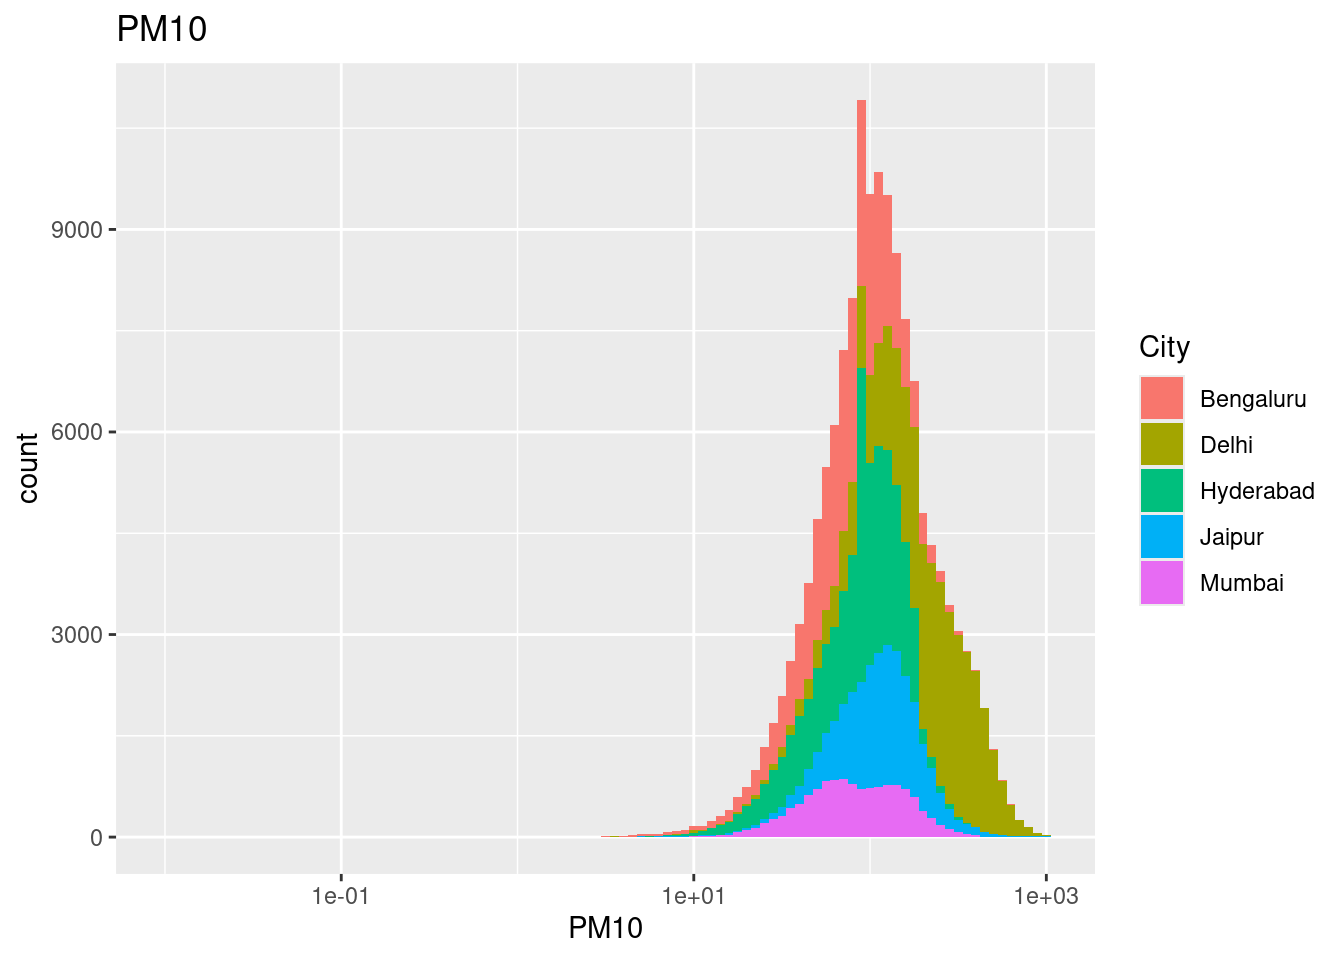
\includegraphics[width=0.7\textwidth]{pm10-by-city.png}
    \caption{PM\textsubscript{10} levels by city}
    \label{fig:pm10_by_city}
\end{figure}


\subsection{Time Series Analysis}

We analyzed whether the time of year affects pollution levels. Although we only present the graph for O\textsubscript{3} pollution, all pollutants exhibit similar behavior: pollution levels tend to be lower during the summer months, from July to September.

\begin{figure}[H]
    \centering
    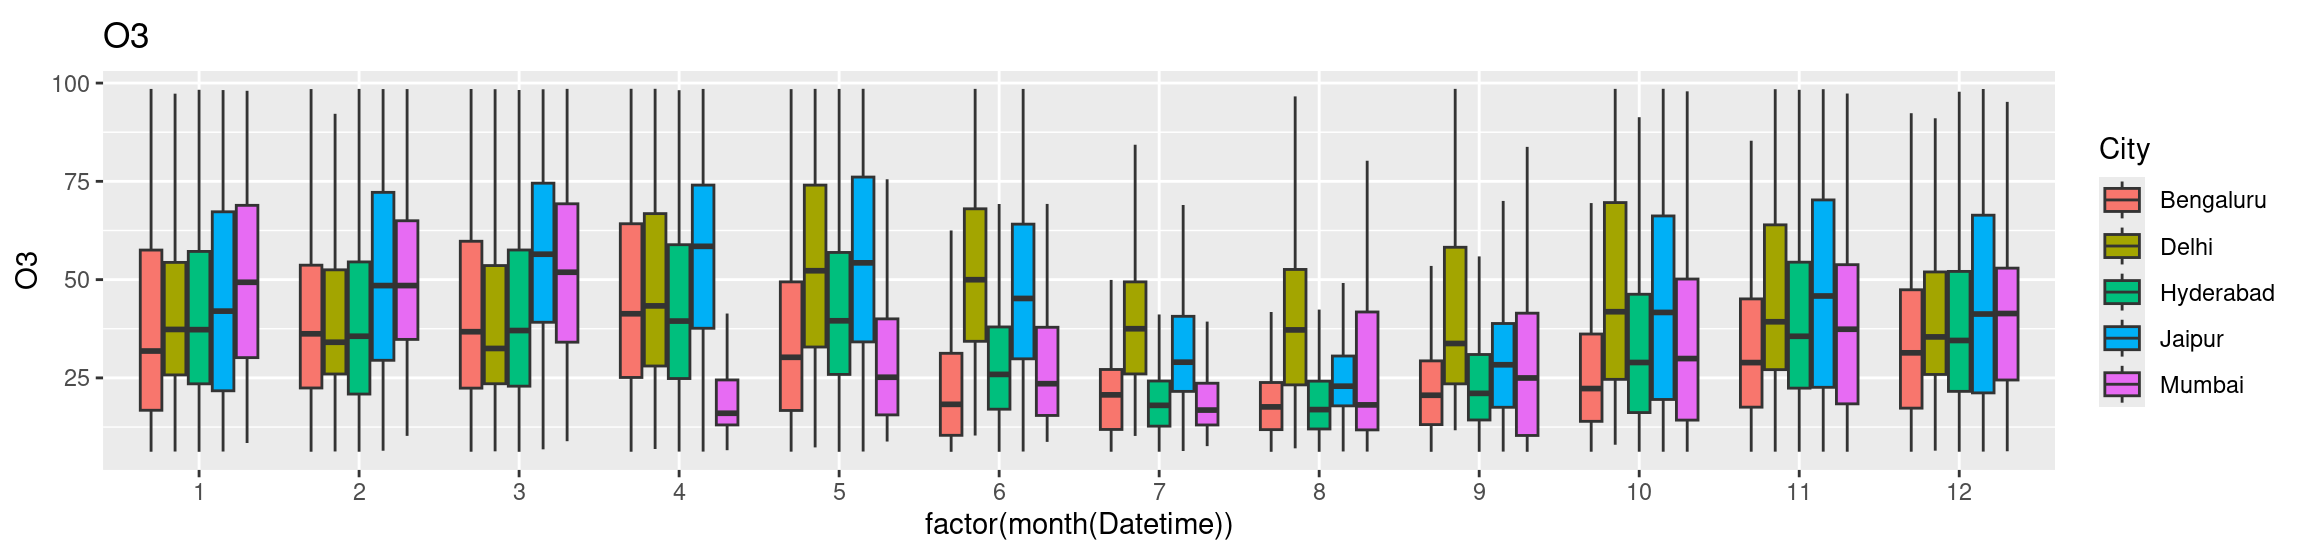
\includegraphics[width=0.7\textwidth]{o3-by-month.png}
    \caption{O\textsubscript{3} levels by month}
    \label{fig:o3_by_month}
\end{figure}

\subsection{Correlation Analysis}

We conducted a correlation analysis to examine the relationships among the weather variables and between the features and response variables.

First, we calculated the correlation matrix for the weather variables:

\begin{figure}[H]
    \centering
    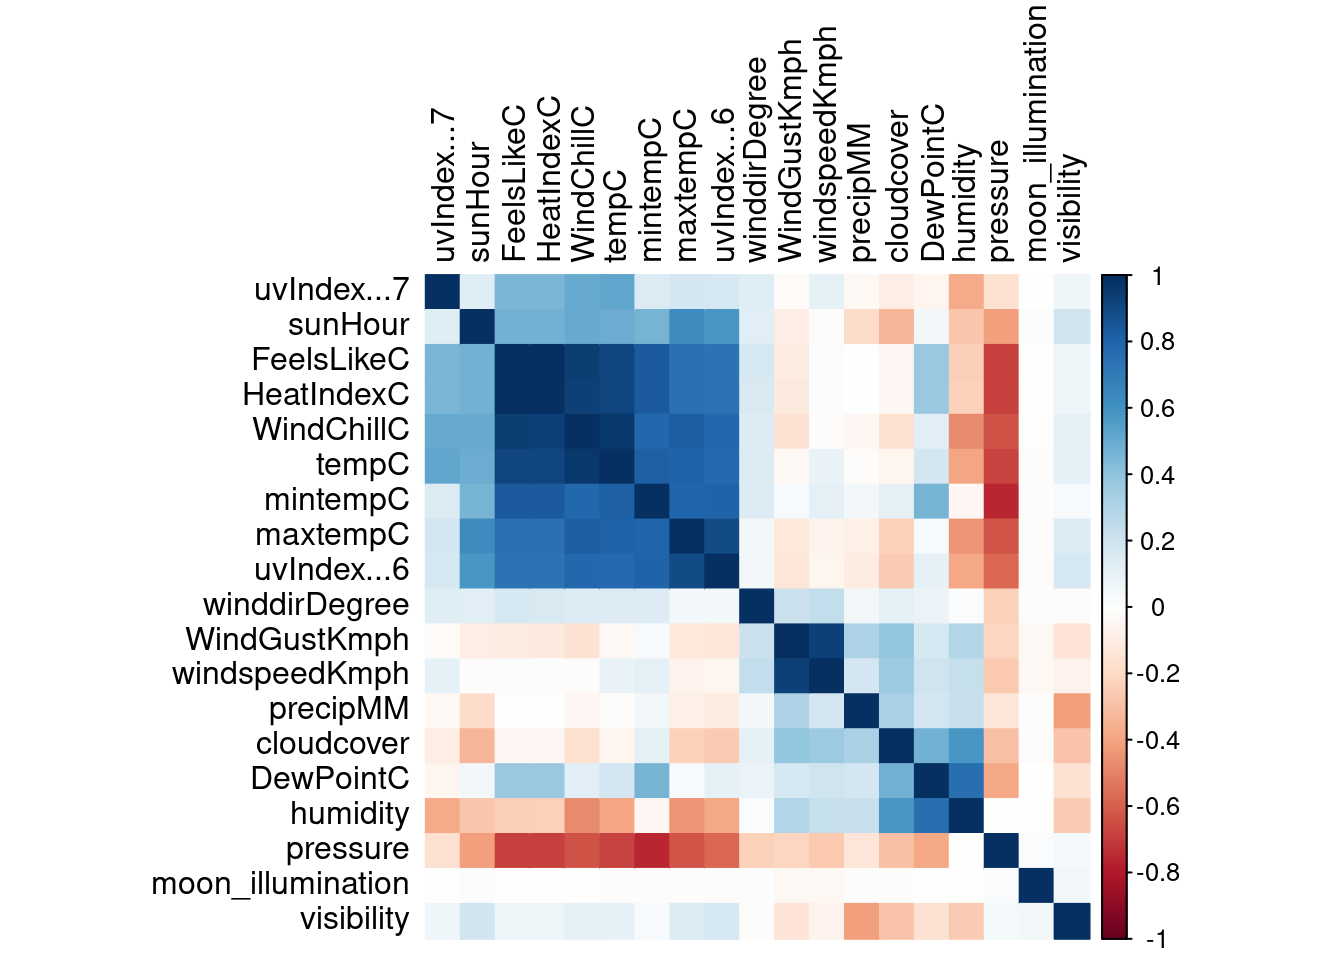
\includegraphics[width=0.7\textwidth]{correlation-matrix.png}
    \caption{Correlation matrix of weather variables}
    \label{fig:correlation_matrix}
\end{figure}

\textbf{Observations:}

The correlation matrix (Figure~\ref{fig:correlation_matrix}) shows that some weather variables are highly correlated with each other. To avoid multicollinearity, we decided to remove variables such as \textit{FeelsLikeC}, \textit{HeatIndexC}, \textit{WindChillC}, \textit{minTempC}, and \textit{maxTempC}, which are highly correlated with \textit{tempC} and are derived from combinations of temperature, humidity, and wind speed. Similarly, \textit{humidity} is correlated with \textit{DewPointC}, and certain UV index variables are highly correlated.

Next, we analyzed the correlation between features and response variables:

\begin{lstlisting}[language=R]
feature_vars <- c(
    "sunHour", "uvIndex", "moon_illumination",
    "DewPointC", "WindGustKmph", "cloudcover", "humidity",
    "precipMM", "pressure", "tempC", "visibility", "winddirDegree", "windspeedKmph"
)

# Calculate the correlation matrix
correlation_matrix <- cor(
    data_merged[, response_vars],
    data_merged[, feature_vars],
    use = "pairwise.complete.obs"
)

# Plot the correlation matrix
corrplot(
    correlation_matrix,
    method = "color",
    tl.col = "black"
)
\end{lstlisting}

\begin{figure}[H]
    \centering
    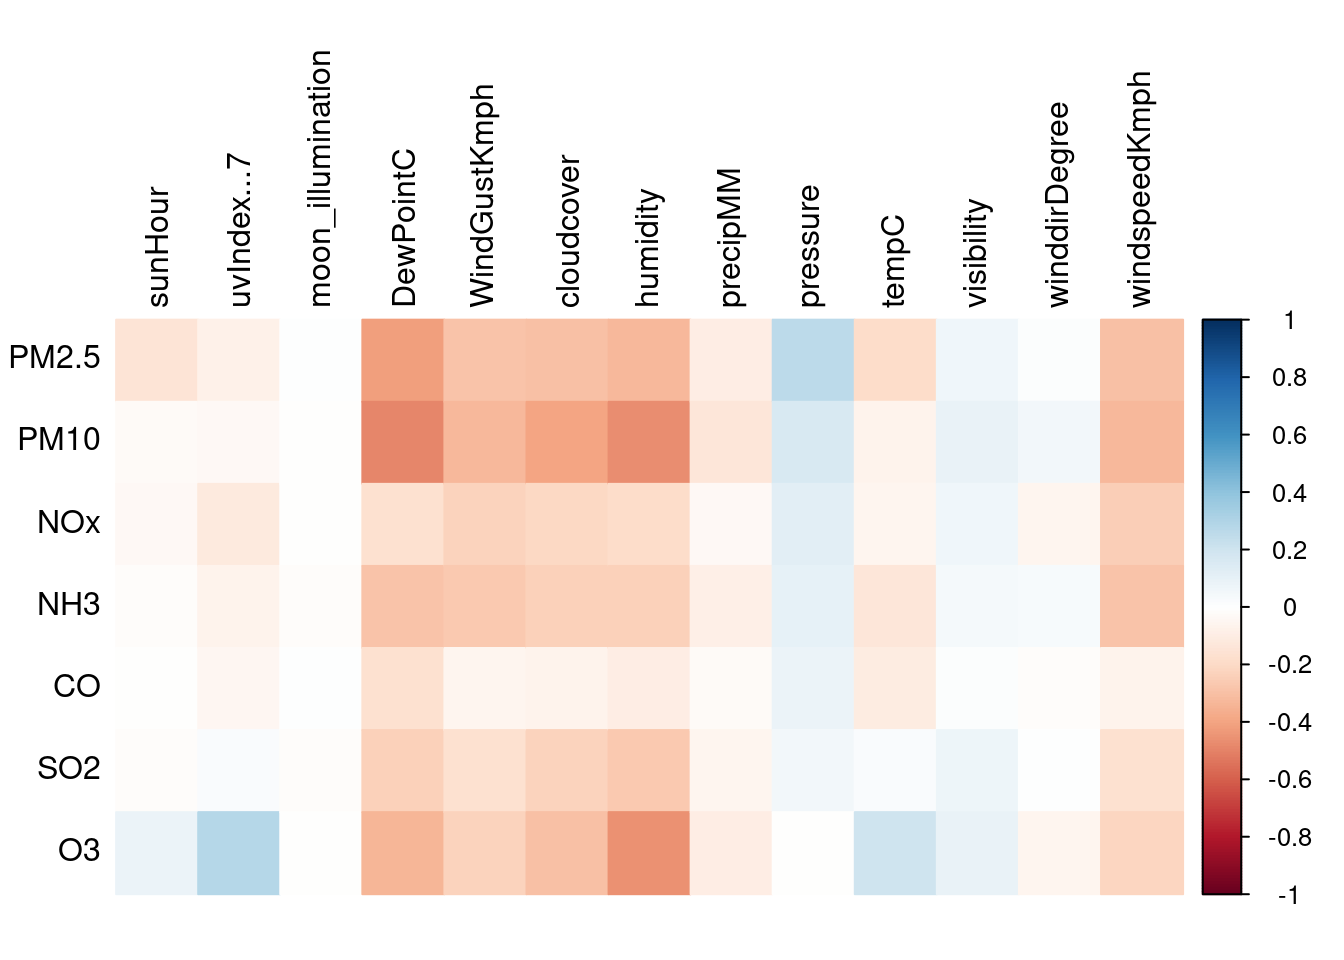
\includegraphics[width=0.7\textwidth]{feature-response-correlation.png}
    \caption{Correlation between features and response variables}
    \label{fig:feature_response_correlation}
\end{figure}

\textbf{Observations:}

The correlation matrix (Figure~\ref{fig:feature_response_correlation}) indicates that the weather variables are weakly correlated with the response variables. However, since we only used a linear correlation measure, there may be non-linear relationships that are not captured in this analysis.

\newpage

\printbibliography

\end{document}
